\documentclass[final,5p,times,twocolumn]{elsarticle}
\usepackage[T1]{fontenc}
\renewcommand{\ttdefault}{lmtt} % Embedded vector Latin Modern Typewriter
\usepackage{microtype,graphicx,booktabs,amsmath,amssymb,array,tabularx,longtable,xurl,placeins}
\usepackage[hypertexnames=false]{hyperref}
\setlength{\emergencystretch}{2em}
\hypersetup{hidelinks,pdfauthor={Chengzhan Li},pdftitle={Reference-Preserving Speculative Decoding on Consumer Systems: Diagnosis, Repair Scope, and Measured Cost},pdfsubject={JSA v0.14.5 author-review manuscript; not submitted}}
\newcommand{\RQtag}[1]{\textbf{RQ#1}}
\makeatletter
\def\ps@pprintTitle{\let\@oddhead\@empty\let\@evenhead\@empty\def\@oddfoot{\hfil\thepage\hfil}\let\@evenfoot\@oddfoot}
\makeatother
\begin{document}
\begin{frontmatter}
\title{Reference-Preserving Speculative Decoding on Consumer Systems: Diagnosis, Repair Scope, and Measured Cost}
\author{Chengzhan Li}
\address{University of Electronic Science and Technology of China\\[2pt]
{\normalfont\ttfamily\href{mailto:chengzhan.li@std.uestc.edu.cn}{chengzhan.li@std.uestc.edu.cn}}}
\begin{abstract}
Speculative decoding changes the numerical history of a quantized runtime as well as its execution cost. When an application requires a fixed ordinary greedy output, the runtime must establish where constraints are needed and whether the qualified design saves time. We connect local state/path diagnosis, phase-scoped repair and measured comparisons with ordinary and matched target-only execution. Natural donor-state crosses on CUDA and Vulkan distinguish current-path, retained-state and interaction effects; a separate B570 fork study shows that immediate agreement can coexist with later divergence. On RTX, a query-layout transformation retains batched projection and feed-forward work. Target prefill and continuation form an inclusion-minimal passing set within a tested four-switch family, and the frozen design qualifies full responses on 24 project-unused inputs. Resident-request speed is 1.742 times ordinary execution; the matched draft-free path already achieves 1.683 times, leaving a 1.035-times speculative increment. Seven tasks regress against matched request time, and one round reverses direction. Wider fixed-capacity drafting and a B570 endpoint repair qualify while losing performance. Auxiliary M4 and 358H cases bound the value of added control and draft-only optimization. These results support a configuration-specific decision process from diagnosis through qualification to cost comparison; repair evidence remains restricted to the tested Qwen3 family.
\end{abstract}
\begin{keyword}
speculative decoding \sep numerical consistency \sep execution state \sep runtime design \sep performance evaluation \sep consumer systems
\end{keyword}
\end{frontmatter}
\section{Introduction}
\label{sec:introduction}
Speculative decoding uses a draft to propose tokens and a target to evaluate several positions at once~\cite{leviathan2023}. On consumer systems, this extra work within a request can amortize target execution when memory capacity and request traffic limit batching across requests. The implementation also changes how the target executes: scalar continuation becomes multi-position verification, cache contents follow a different history, and rejected positions require reconciliation. A valid sampling rule therefore leaves two practical questions open: does the quantized runtime reproduce the required output, and does it reduce the cost of producing it?

We study systems in which ordinary greedy decoding under a fixed runtime configuration defines the reference. Such a requirement arises in regression tests and applications that need repeatable outputs. Reference preservation means matching the registered token sequence or endpoint; it does not establish that the answer is functionally correct or that every intermediate floating-point value is identical. The runtime designer must choose where to enforce consistency and then measure the resulting cost. A constraint can repair one input while breaking another, or recover the output at the expense of the intended acceleration.

The visible token prefix does not determine the necessary constraint. Two executions can emit identical tokens while retaining different key/value (KV) values, pending tokens or sampler history. Their next decision can follow the retained state, the current execution recipe, or an interaction between the two. Conversely, different scores can produce the same immediate greedy decision while later outputs diverge. Distinguishing these cases helps decide whether to constrain state formation, current verification, or both.

A repair may improve the target path before a draft is added. Comparing repaired speculation only with ordinary decoding measures the combined deployment change. A matched target-only execution, using the repaired path without a draft, measures how much additional benefit speculation supplies. Both paths must be executed and charged under the same output requirement; acceptance rates and target-call counts cannot replace their measured costs.

An RTX continuation intervention repairs one task and regresses another, leaving aggregate reference agreement unchanged. A later phase-scoped attention implementation qualifies full responses on 24 inputs unused in the accessible project history. Its resident-request speed is $1.742\times$ ordinary decoding, but the matched draft-free path already achieves $1.683\times$; adding speculation gives $1.035\times$. A distinct B570 implementation preserves its registered endpoint while remaining substantially slower than both draft-free baselines. We organize the study around three questions:
\begin{enumerate}
\item \RQtag{1}, diagnosis: does the observed deviation follow retained state, the current recipe, or their interaction?
\item \RQtag{2}, repair: which phase constraints preserve the reference within a defined implementation family?
\item \RQtag{3}, cost: after qualification, what benefit remains against ordinary decoding and the matched target path?
\end{enumerate}

The contribution is a linked diagnosis, repair and cost evaluation within explicit output contracts. Natural donor-state crosses with own-path controls distinguish local state, path and interaction effects on CUDA and Vulkan; a separate same-state B570 fork study establishes the limits of immediate agreement. The RTX query-layout transformation retains batched projection and feed-forward work, and a complete four-switch factorial identifies a sufficient target-phase scope within the tested family. Measured ordinary/matched/speculative comparisons separate the full deployment gain from the speculative increment. B570 supplies a qualified-but-slower counterexample, while the auxiliary M4 and 358H cases delimit the value of added control and draft-only optimization.

The study concerns runtime design and finite qualification. Its crosses are offline experiments, and the repair remains specific to the tested Qwen3 family and configurations. Sections~\ref{sec:runtime} and~\ref{sec:methods} define the implementation context and measurement contracts; Sections~\ref{sec:diagnosis}--\ref{sec:cost} answer the three questions. Section~\ref{sec:implications} draws the resulting design choices and states their limits. The supplement retains campaign details, historical results and the complete evidence trail.

\section{Runtime Architecture and Research Context}
\label{sec:runtime}
\subsection{Execution as a stateful transaction}
A speculative iteration advances a committed prefix through drafting, target verification and reconciliation. The draft proposes up to $k$ tokens; the target evaluates the pending token and proposal positions, often in a caller batch containing several tokens. Acceptance, correction and a possible bonus token determine the committed output. Rejected positions must be removed or reconciled before the next iteration, and stopping follows the registered EOG and cap rule. Figure~\ref{fig:architecture} connects these operations to the state and phase controls studied here.

Target and draft retain distinct state (Figure~\ref{fig:architecture}A). KV ownership, logical positions, pending logits or tokens, sampler history and loop counters connect successive calls. A token can already be sampled and accepted into the sampler while still awaiting evaluation into the cache. Repeating or omitting either event changes the transaction. The early intervention frontends therefore preserve pending and sampler state as well as KV. The later B570 candidate binds phases within one target context and live sampler; the measured RTX candidate uses no state transplant.

\begin{figure*}[t]
\centering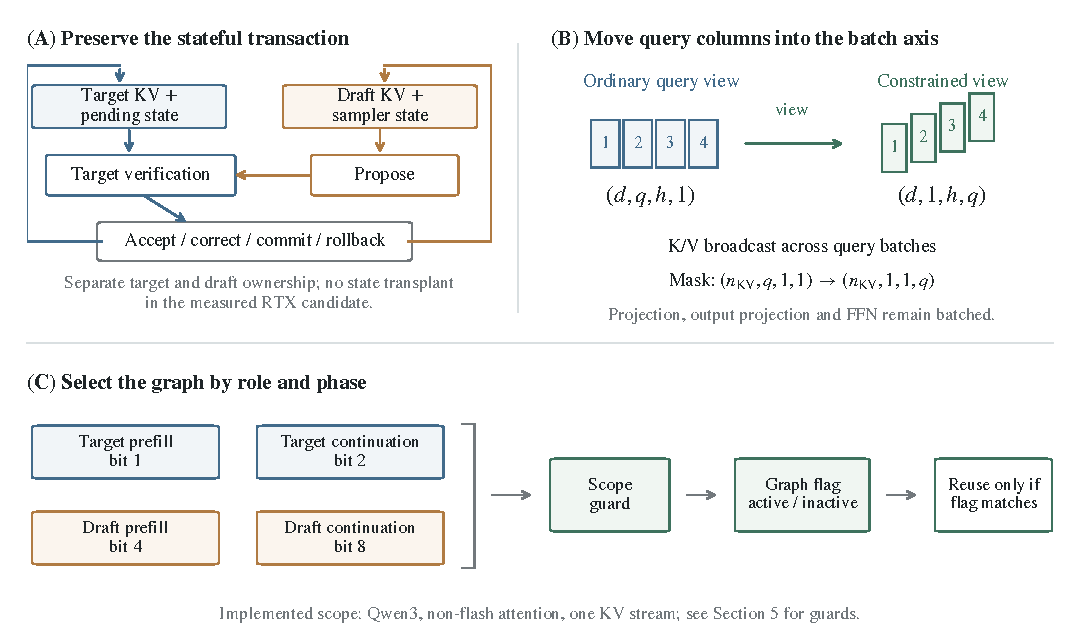
\includegraphics[width=\linewidth]{figures/figure_1_architecture.pdf}
\caption{State ownership and implemented consistency controls. (A) Target and draft keep distinct state through proposal, verification and reconciliation. (B) The RTX query view moves query columns into the batch axis while retaining batched projection and FFN work; numbered tiles are illustrative. (C) Role and phase select the query-batch graph flag, which must also match for topology reuse. The measured RTX candidate uses no state transplant. Section~\ref{sec:repair} defines the transformation and its implementation guards.}
\label{fig:architecture}
\end{figure*}

Microbatch capacity UB limits how the backend partitions a caller batch. It is distinct from $k$, the occupied query count and the frontend's output reservation. A UB2 caller may contain only one continuation token; increasing $k$ can reduce caller count while increasing the number of micrographs; changing output reservation can alter the recipe without changing UB. Capacity, occupied queries and output reservation must therefore be distinguished when interpreting diagnostic crosses and performance counters.

The implementations use pinned llama.cpp releases and private frontends~\cite{llamacpp}. The late RTX path uses Qwen3-8B and Qwen3-0.6B~\cite{qwen3}, both Q8\_0, with non-flash CUDA attention. Its transformation uses existing ggml views and operations, with no new CUDA arithmetic kernel or acceptance rule. B570 uses Vulkan and a distinct phase-binding frontend. Historical Metal and OpenVINO cases retain their own contracts. Because hardware, backend and frontend vary together, these cases compare execution designs rather than hardware alone.

\subsection{Reference preservation and determinism}
Our requirement fixes an ordinary path and an output endpoint. A matching token sequence may still have different logits or cache values, while a repeat-stable candidate can consistently disagree with the reference. Numerical-consistency work explains how execution shapes and reductions affect this distinction. Batch-invariant inference constrains reduction strategies across batches~\cite{thinkingmachines}. LLM-42 combines decode--verify--rollback, padded verification shapes and replacement of decoded KV entries with verifier entries; it permits different consistent strategies for prefill and decode~\cite{llm42}. Stage-Replay examines fixed-prefix precision controls and bidirectional cache transplantation~\cite{stagereplay}. Vosti specifies and verifies deterministic system behavior~\cite{vosti}, and MarginGate uses margin-triggered verification with repair of confirmed mismatches~\cite{margingate}.

We use these consistency and verification principles to connect natural donor-state diagnosis to a query-layout and phase design, then test finite native-output qualification and paid cost. Table~\ref{tab:related} summarizes this scope. We do not implement a same-contract comparison with LLM-42, Stage-Replay or Vosti, so the results establish no speed or preservation advantage over those methods.

\begin{table*}[t]\centering\small
\caption{Research context and additional evidence in this study. The cited methods are not same-contract performance baselines.}
\label{tab:related}
\begin{tabularx}{\linewidth}{@{}p{.23\linewidth}XX@{}}\toprule
Prior work & Established basis & Additional evidence here\\\midrule
Batch-invariant inference; LLM-42~\cite{thinkingmachines,llm42} & Reduction/shape consistency; verified tokens and KV reconciliation & Qwen3 query views and phase dispatch, finite qualification, and ordinary/matched paid costs\\
Stage-Replay; Vosti~\cite{stagereplay,vosti} & Fixed-prefix state intervention; specified system determinism & Natural donor $\times$ current-recipe crosses with shams; output qualification in a tested implementation family\\
Consumer cost anatomy; Performance or Illusion?~\cite{lossless,illusion} & Backend verification cost and limits of performance proxies & Qualified fixed-UB width failure and separation of target-path from speculative request gains\\\bottomrule
\end{tabularx}
\end{table*}

\subsection{Performance and heterogeneous execution}
Prior work uses heterogeneous placement and draft-budget control to improve execution. Dovetail and DuoDecoding exploit complementary CPU/GPU capabilities~\cite{dovetail,duodecoding}; TurboSpec and BanditSpec adapt speculation to execution conditions~\cite{turbospec,banditspec}. The published HeteroSpec studies contextual heterogeneity in verification allocation~\cite{aclheterospec}. We require preservation of a selected ordinary output and measure whether the transformation reduces cost.

Lossless but Not Free examines consumer backend cost and cache choreography when verification fails to amortize target work~\cite{lossless}. Performance or Illusion? shows why reductions in apparent decoding work do not guarantee production-engine performance~\cite{illusion}. We add reference qualification and the matched draft-free comparator to that decision. M4 control and 358H offload illustrate separate cost limits; neither replicates the RTX repair.

\section{Study Design and Measurement Contracts}
\label{sec:methods}
\subsection{Systems, inputs, and evidence roles}
The principal cases use the contracts in Table~\ref{tab:contracts}. All final targets are Qwen3-8B: changing the device, draft representation or backend does not create a second target family. HumanEval~\cite{humaneval} and sanitized MBPP~\cite{mbpp} supply coding inputs; M4 also uses a prospective Spec-Bench partition~\cite{specbench}. Prompt construction remains campaign-specific. The measured output property is reference reproduction, not benchmark test-pass accuracy.

\begin{table*}[t]\centering\small
\caption{Principal study contracts. Each case processes one request at a time. Historical text checks, which are weaker than direct-ID qualification, are retained separately in the supplement.}
\label{tab:contracts}
\begin{tabularx}{\linewidth}{@{}p{.17\linewidth}p{.26\linewidth}XX@{}}\toprule
Case & Runtime/model setting & Output and exposure & Paid interval\\\midrule
RTX expansion & 5070 Ti Laptop; CUDA; Q8\_0 target/draft; private b10839-based frontend & Full response through EOG/cap128; 24 project-unused MBPP, four repeats & Server generation; resident HTTP request\\
B570 repair & Arc B570; Vulkan; Q8\_0 target/draft; phase-binding frontend & First-EOG/cap128 endpoint; 15 project-unused inputs, two repeats & Native generation; whole request; host return\\
M4 runtime & MacBook Air M4; Metal; Q8\_0 target/draft & Direct generated IDs; prospective 30 HumanEval plus 30 Spec-Bench, three repeats & Registered post-prefill runtime interval\\
358H stateful & Arc B390 Vulkan target; symmetric INT4 OpenVINO CPU/NPU draft & Direct IDs; 30 prompts, three repeats per draft condition & Registered stateful interval and target-work accounting\\\bottomrule
\end{tabularx}
\end{table*}

The late RTX and B570 candidates use non-flash attention, greedy sampling and separately frozen capacities, phase settings and runtime/model bindings (Supplement \S S1 and \S S5.2). Their campaigns remain separate. The five evidence roles are: prediction reproduces native behavior; selected-boundary crosses diagnose local dependence; exposed probes select a repair; a frozen recipe is checked on project-unused inputs; and separate paid sessions measure qualified cost. Repetitions describe stability and cost variation. Forks and within-request decision events belong to their parent tasks and do not increase the independent input count.

For the RTX expansion, eligibility and the recipe were frozen before new reference outputs were generated. The exposure audit excluded previously executed or ambiguous inputs and selected 24 MBPP tasks from 224 eligible candidates. No eligible unused HumanEval inputs remained at that stage, so a pre-output amendment selected MBPP. Project-unused means absent from accessible project execution records, not unseen during training. The panel becomes exposed when reused for width studies and later CPU analyses. B570's 15-input panel follows its own accessible-history audit; omitted RTX bulk records were not independently rescanned.

\subsection{Registering the output requirement}
Let $R(x)$ denote ordinary output under fixed weights, tokenizer, prompt formatting, sampler, runtime, backend and stopping rule. RTX qualification compares the full response array, length, terminal ID and stop reason, and checks reference repeat stability. The expansion contains a complete $24\times4\times4$ task/condition/repetition matrix: 384 rows and 96 qualified responses per condition. Reference lengths range from 11 to 128 IDs; 23 tasks stop at EOG and one at the cap.

B570 retains IDs through the first runtime EOG or token 128, whichever comes first. A speculative response can satisfy this endpoint requirement while containing additional raw suffix IDs. Those IDs remain charged. Endpoint equality, raw-array equality and unknown historical raw comparisons are reported separately. Historical re-tokenized-text checks retain their original weaker contract (Supplement \S S1).

A latency ratio qualifies as a reference-preserving speedup only after the output gate passes. A shorter divergent response does not qualify, and repeat stability alone cannot certify agreement with $R$. The finite checks establish neither functional correctness nor equality of all intermediate values or arbitrary future outputs.

\subsection{Controlled state and current-recipe crosses}
At a naturally reached boundary, express the decision as
\begin{equation}
d=F(p,s,e),
\label{eq:decision}
\end{equation}
where $p$ is the committed prefix, $s$ the retained runtime/numerical state and $e$ the current execution recipe. Cross two naturally formed donors $s_0,s_1$ with recipes $e_0,e_1$, holding the registered prefix and current logical input fixed. In the resulting matrix, a within-row change is a current-recipe effect for that donor; a within-column change is a donor-state effect for that recipe. Dependence on one factor only under a particular value of the other indicates a local interaction. Token IDs are categories; their numerical differences are not effect sizes.

A valid cross requires consistent cache ownership and positions, faithful restoration, and compatible pending and sampler semantics. Own-path shams restore each donor under its native recipe and compare with uninterrupted execution. Natural donors use online proposals, without feeding future reference answers or a recorded proposal tape into the candidate. Earlier sealed-proposal prediction studies answer a separate reproduction question (Supplement \S S2.1). The selected cuts probe known sensitivity; they do not estimate its prevalence or provide a complete counterfactual suffix for every cell.

\subsection{Two paid baselines and task-level estimation}
Let $M$ be target-only execution on the repaired path and $C$ speculation on that path. Together with ordinary $R$, they distinguish the deployment change $R/C$, target-path change $R/M$ and incremental draft benefit $M/C$. Each baseline is executed and charged. $R$ is the registered comparator; it is not a proven optimum over ordinary implementations.

For late RTX and B570, first take each task's median absolute time in each condition, then form its baseline/candidate ratio. For $n$ complete task pairs,
\begin{equation}
S_{b/c}=\exp\left[\frac{1}{n}\sum_{i=1}^{n}\log\left(t_{i,b}/t_{i,c}\right)\right].
\label{eq:gm}
\end{equation}
A ratio above one favors the denominator path. For common tasks and this aggregation,
\begin{equation}
S_{R/C}=S_{R/M}S_{M/C}.
\label{eq:identity}
\end{equation}
This multiplicative identity cannot allocate attention, KV, synchronization or host cost. M4 retains its frozen estimator and random streams; 358H uses a median of paired ratios before the task geometric mean, a different estimator.

RTX ordinary-reference ratios are a later CPU reanalysis of the same paid records; the expansion originally emphasized matched comparisons. Descriptive 95\% intervals resample the 24 task-median ratios with 10,000 common index resamples, NumPy PCG64 seed 20261008 and linear/type-7 quantiles. The earlier bootstrap convention remains in Supplement \S S4.1. Task resampling does not estimate session or day variation, and round-specific geometric means are reported separately from the task-median estimator.

The RTX server-generation field \texttt{predicted\_ms} charges draft and verification work between its timestamps, excluding initial prompt work and first sampling and potentially final bookkeeping. Resident-request time covers non-streaming HTTP response receipt and parsing. Loading, warmup, boundary telemetry and shutdown are excluded; post-response asynchronous cleanup is not certified inside this interval. Their difference is not a measured host component. B570's native-generation, whole-request and host-return boundaries are defined separately in Supplement \S S5.4. Unlike timers are not pooled into a platform ranking.

\section{Locating the Consistency Boundary (RQ1)}
\label{sec:diagnosis}
\subsection{A repair and a regression under the same intervention}
The continuation experiment tests whether a local path change can recover the reference. The RTX intervention changes target continuation from UB2 to UB1 while retaining prefill, draft settings and caller grouping. On 19 exposed HumanEval tasks, the predictor reproduces both native conditions in all 57 repeated complete arrays. HumanEval/15 repairs, /25 regresses and /18 remains divergent, leaving reference agreement at 51/57 in both conditions. The unchanged aggregate conceals opposing task effects, so continuation-only control does not satisfy recovery without regression.

A separately selected 24-task MBPP panel reaches 72/72 prediction/native agreement in each condition, but only 66/72 reference agreement. MBPP/304 remains a divergent 47-ID response while changing token 488 to 481 at zero-based position 33. Accurate prediction of a changed response does not establish reference recovery. We therefore examine retained state and the current call separately.

\subsection{Natural donor state crossed with the current call}
In Figure~\ref{fig:cross}, rows select naturally formed donor states and columns select the current recipe at a shared committed prefix. Horizontal changes expose current-path dependence; vertical changes expose retained-state dependence. The displayed IDs label decisions rather than numerical distances. A change confined to one donor/recipe pairing indicates an interaction. Own-path shams check that restoration itself preserves the native decision.

For RTX, N0 and N1 denote the native baseline and continuation-intervention histories. Four exposed HumanEval probes yield 24 donors, 48 state/current-path forks and 24 shams across repetitions. Donors preserve actual pending state, cache positions and sampler history. The shams pass and forking leaves the original context unchanged. At /15's 13-token cut, either donor gives 9147 under current UB2 and 4199 under UB1 at the third submitted decision (Figure~\ref{fig:cross}A). The local decision follows the current path. At /25's four-token cut, only the N1-donor/current-UB1 cell changes, producing the sequence 271,750,8168 rather than beginning with 1406 (Figure~\ref{fig:cross}B). This is a local interaction between state and path. The selected /18 and /31 cuts are discrete nulls, which do not establish invariance over their remaining trajectories.

\begin{figure*}[t]
\centering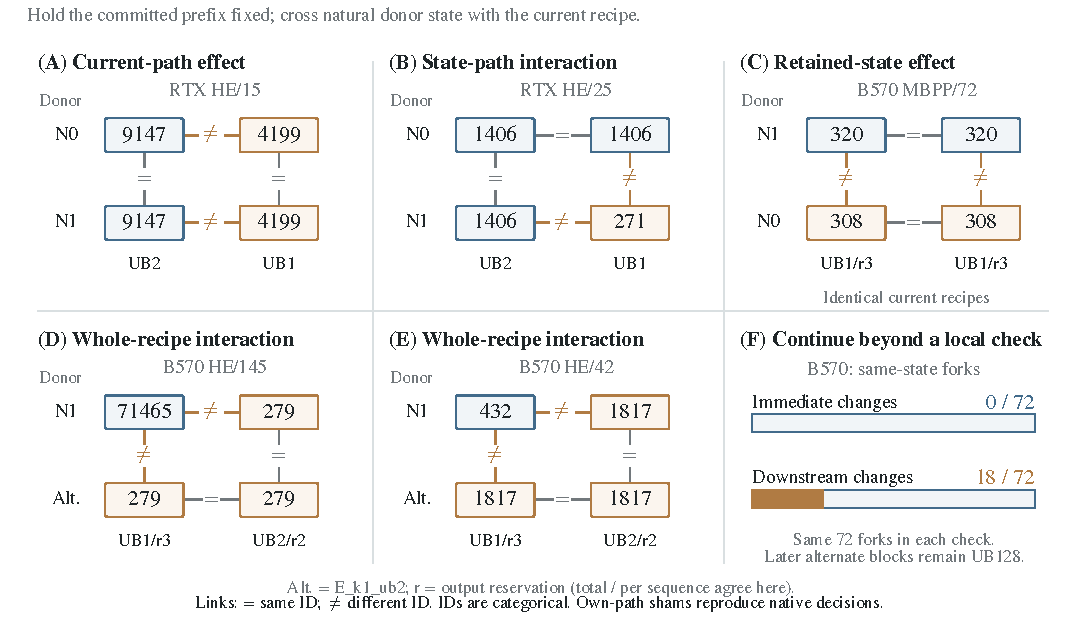
\includegraphics[width=\linewidth]{figures/figure_2_natural_crosses.pdf}
\caption{Three local dependencies and the limit of a local check. Rows select natural donor states; columns select the current recipe. Token IDs are categorical; filled tiles group equal IDs, and links mark equality or difference between adjacent cells. (A) RTX /15 follows the current path. (B) RTX /25 and (D,E) B570 HumanEval show interactions. (C) B570 MBPP/72 follows retained state under identical UB1/reservation3 columns. The B570 HumanEval columns change UB and output reservation together. N0 in (C) is the ordinary donor; Alt. in (D,E) is the cross recipe E\_k1\_ub2. Here $r$ denotes output reservation; the two HumanEval recipes use UB1/$r=3$ and UB2/$r=2$. Own-path shams pass. (F) A separate B570 study finds 0/72 immediate but 18/72 downstream changes under sustained alternate UB128 continuation; it does not isolate a single-block aftereffect.}
\label{fig:cross}
\end{figure*}

All 12 prompt-KV donor comparisons agree, whereas 70 of 72 generated-prefix K/V tensor comparisons differ; the tested first-layer K/V remain equal. The discriminating /15 bonus row is itself a single-token microbatch under either history. Its final nominal shape alone therefore cannot explain the decision: inputs and preceding state formation also matter. The evidence motivates attention-related controls without isolating a unique kernel cause. Auxiliary short continuations and their 1,278 forwards are diagnostic work, not a paid performance panel.

\subsection{One unchanged block does not certify the remaining trajectory}
A separate B570 experiment forks the same live state, with byte-checked KV, at the first eligible verification block after at least 64 committed IDs. It processes that block under UB1 or UB128. Twenty-four reserved prompts and three repetitions produce 72 eligible forks. Every paired raw score record changes, yet immediate top-1 IDs and acceptance decisions remain equal across 195 paired decision events: no execution or task changes its immediate decision.

Complete committed-ID trajectories in Figure~\ref{fig:cross}F differ in 18/72 executions from six of 24 tasks. Later alternate blocks continue to use UB128, and proposals evolve under the accepted history. This result concerns a sustained continuation policy, not one altered block followed by restoration. Qualification must therefore check the registered output beyond the sampled block: a local discrete null can coexist with later divergence, and score movement alone does not predict an immediate decision change. Neither the 72 forks nor the 195 internal events constitute additional independent tasks.

\subsection{B570 crosses identify a whole-recipe boundary}
For B570, N1 labels the repaired prior frontend. The figure labels the alternate HumanEval donor Alt. (E\_k1\_ub2) and the ordinary MBPP/72 donor N0. Neither denotes the later phase-binding candidate. These crosses test whether the RTX diagnostic distinction remains useful in a different runtime. Three tasks in six repeated contexts provide 12 own-path shams and 24 auxiliary target cells. Restored states retain checked byte contents, sequence-zero ownership and logical positions. At HumanEval/145's prefix 56, the selected matrix is $[(71465,279),(279,279)]$; at /42's prefix 73 it is $[(432,1817),(1817,1817)]$ (Figure~\ref{fig:cross}D,E). Both show a local interaction. At MBPP/72's prefix 40, $[(320,320),(308,308)]$ varies only with donor state, under identical current UB1/output-reservation-3 columns (Figure~\ref{fig:cross}C).

The HumanEval recipes change microbatch capacity and output reservation together, so the factor tested is the whole recipe. These crosses do not isolate UB or transfer the RTX repair to Vulkan. Full counterfactual continuations for each cell are unavailable; the subsequent B570 candidate undergoes its own native endpoint qualification. The greedy sampler history, clone metadata and shams support the tested restoration, while opaque sampler bytes and general stochastic-state restoration remain outside that check. At the same committed prefix, local path, state and interaction dependence can require different control placements.

\subsection{Prediction and simple execution constrain added machinery}
Prediction fidelity alone does not establish an online repair mechanism. B570 prospective prediction matches 72/72 native arrays on a reserved 24-task cohort even though reference agreement is 60/72. RTX's initial target-only batched-path predictor reaches 24/36 and fails its frozen 36/36 gate, so no reserved inference follows. A later independent-proposal replay obtains H2/native and reference-only/native agreement of 72/72, again with 60/72 reference agreement. The later study resolves the earlier reproduction interface, but neither result establishes cheap online correction.

On the 19 RTX tasks, draft-free $U_2$ reproduces all 57 intervention $N_1$ arrays and stop boundaries, including /15's repair and /25's regression. It needs no draft, transplant, proposal tape or reference answer. This establishes output equivalence, without a speed claim or demonstrated equality of live logits/KV.

Offline screening provides no supported evidence-acquisition advantage over direct enumeration. RTX direct enumeration and proxy screening both abstain after 114 record equivalents beyond common acquisition; B570 direct verification requires 72 and proxy screening 144. Unknown counterfactuals remain unknown. These are evidence-acquisition counts, not latency measurements. RQ1 identifies local diagnostic distinctions; an automatic repair selector remains unvalidated.

\section{Phase-Scoped Implementation and Qualification (RQ2)}
\label{sec:repair}
\subsection{Constraining attention while retaining batched work}
The RTX design targets the attention graph rather than serializing the whole network. An initial implementation builds one non-flash Qwen3 attention subgraph per query and concatenates the results. The later query-batch implementation represents query columns in the ggml batch dimension, allowing existing operations to process them in parallel while preserving one-column query structure. Projection, output projection and feed-forward computation remain batched (Figure~\ref{fig:architecture}B).

After the existing query/key/value permutations, the supported single-KV-stream query has dimensions $(d,q,h,1)$. A \texttt{ggml\_view\_4d} reinterprets it as $(d,1,h,q)$, preserving the source strides and assigning the original query-column stride to the new batch axis. Shared K/V broadcast across query batches; the mask view changes from $(n_{\mathrm{KV}},q,1,1)$ to $(n_{\mathrm{KV}},1,1,q)$. Existing key-query multiplication, softmax, value multiplication and contiguous recombination perform attention. The design retains the tested scalar-query computation structure locally while preserving parallel work elsewhere; it adds no new backend arithmetic.

Implementation guards admit Qwen3 non-flash attention, one KV stream and compatible mask dimensions, with no attention bias, sinks or MLA value projection. The initial limit is four queries; a later width build extends the admitted graph to eight. Native qualification is required within those guards, and unsupported model graphs, precisions or backends inherit no preservation claim.

\subsection{Phase dispatch and graph reuse are part of the implementation}
The transformation must be active in the intended phase, including when diagnostic capture is disabled. A process-fixed mask and thread-local guard select target prefill/continuation bits 1/2 and draft prefill/continuation bits 4/8 (Figure~\ref{fig:architecture}C). The guard restores the prior active state on exit and executes before the capture-disabled fast path returns to native decoding. Diagnostic settings therefore cannot silently bypass the constraint.

The active query-batch flag is copied into graph parameters and context. Reuse is rejected if it differs from the cached topology key, preventing a phase-layout mismatch even when ordinary microbatch fields agree. A new prompt resets the phase to prefill. Role and phase therefore control graph construction and reuse directly.

Qualification checks captured multi-query nodes and capture-on/off behavior; paid capture-off sessions omit observer metadata and forced witness synchronization. The optional target-state-move branch is inactive in the expansion configuration. The measured candidate charges native drafting, verification and reconciliation without that transplant. Implementation details and timer boundaries are retained in Supplement \S S3.1.

\subsection{The finite phase family}
The factorial tests which phases require the query-batch constraint in this implementation. Figure~\ref{fig:phase}A tests all 16 masks at $k=3$/UB4 on four exposed HumanEval probes, twice each: 128 requests. Outputs and stop boundaries are repeat-stable. Masks 3, 7, 11 and 15 pass the complete panel. /15 and /31 pass every mask, /25 needs at least one target-phase bit, and /18 needs both; draft bits do not change this pattern.

\begin{figure*}[t]
\centering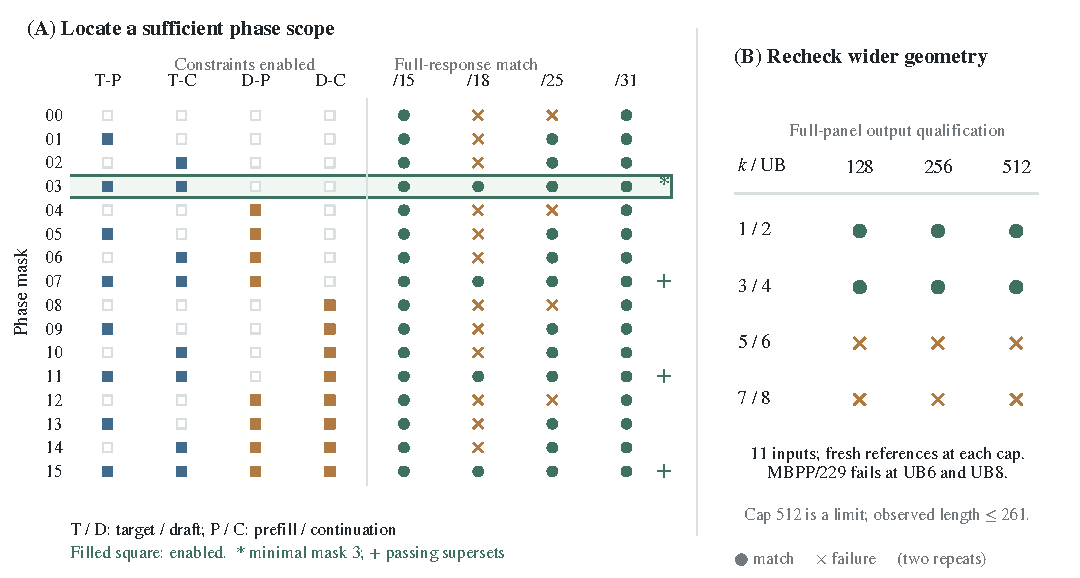
\includegraphics[width=\linewidth]{figures/figure_3_phase_matrix.pdf}
\caption{Qualification of phase scope and geometry. (A) All 16 masks at $k=3$, UB4 and cap128 on four HumanEval probes, with two repetitions (128 requests). Filled squares enable constraints; circles indicate full-response matches and crosses failures. Passing masks are 3/7/11/15; mask 3 is inclusion-minimal within this four-switch family. (B) A separate 11-input panel changes $k$ and UB jointly at caps128/256/512, using fresh scalar references and two repeats. MBPP/229 fails at UB6/8 while matched controls pass. Actual output length reaches at most 261; the earlier HE/18 target-only failure is outside this panel.}
\label{fig:phase}
\end{figure*}

Mask 3 alone has no passing strict subset, making it inclusion-minimal in the tested four-switch family. This selects a sufficient target-phase scope, not a universal requirement on every input or implementation. Acceptance, cache ownership and stopping still need to preserve the transaction. The factorial also uses different geometry from the earlier UB2/UB1 intervention, so /15's all-mask agreement does not negate that path effect.

A smaller scope need not be faster. In a separate 19-task, six-repetition cost panel, mask 3 gives $1.278\times$ generation and $1.113\times$ request speed against matched target-only. Removing draft constraints from mask 15 adds only $1.004\times$ generation speed, with descriptive interval $[0.998,1.009]$, below the frozen $1.03\times$ extra-generation gate. The later 24-input expansion gives $1.015\times$ over mask 15. Scope selection therefore follows qualification, with its cost assessed separately.

\subsection{Frozen inputs and geometry boundaries}
The frozen mask-3/$k=3$/UB4 recipe qualifies all 96 candidate responses on the 24-input expansion. Matched target-only and mask-15 speculation also qualify. This extends the repair from exposed probes to a separately frozen panel, within the same model family and configuration.

Figure~\ref{fig:phase}B tests the geometry boundary on an independent 11-input panel at $(k,\mathrm{UB})=(1,2),(3,4),(5,6),(7,8)$ and caps128/256/512, using fresh scalar references and two repeats. The first two pairs qualify; MBPP/229 fails at both wider pairs across all caps and repetitions while matched controls pass. The earlier HumanEval/18 wide target-only failure remains a separate boundary outside this denominator. The longest observed reference has 261 IDs, so cap512 is a limit rather than evidence of a 512-token trajectory.

At MBPP/229's common 47-token prefix, crossing naturally retained ordinary and constrained states under two current UB6 layouts changes the EOG decision with the donor. Current layout changes continuous scores without a separate discrete flip; four own-path shams pass. This local retained-state effect explains why changing only the current layout at that boundary is insufficient, without identifying a unique cause of all width failures. Two cap contexts repeat one task boundary. The joint $k$/UB sweep remains distinct from the fixed-UB draft-width cost experiment in Section~\ref{sec:cost}.

\subsection{A separate B570 implementation and qualification scope}
The B570 candidate uses a different control interface: it forms target state with the ordinary prompt caller and output reservation, samples the pending token once, then binds continuation from UB128 to UB1 in the same context and live sampler. A private API synchronizes, changes capacity and requests scheduler reservation under a frozen context/batch/sequence contract. Instrumented checks compare serialized KV across binding; paid capture-off requests omit witness readbacks. The existing $k=2$, draft-UB1 accept/bonus/rollback loop remains.

The candidate qualifies 12 development requests, 112 requests on 56 exposed inputs and 30 requests on 15 project-unused inputs under its endpoint contract. It removes the old second context and three witness readbacks but does not implement the RTX query-layout transformation. Earlier B570 repair produced a local long-panel gain yet failed MBPP/72 on a new-input panel and five UB2 alternatives (Supplement \S S5.1). The later same-context binding provides a separately qualified repair whose cost is assessed in the following comparisons.

\section{Does the Qualified Design Pay? (RQ3)}
\label{sec:cost}
\subsection{RTX: deployment gain and speculative increment}
The RTX comparison separates two decisions before measuring their benefit (Figure~\ref{fig:cost}A). Ordinary target-only $R$ uses mask 0/UB1; matched target-only $M$ uses mask 3/UB4; speculative $C$, also denoted $C_3$, adds a draft at $k=3$ on that path. A fourth condition, $C_{15}$, constrains all phases. Each of four balanced rounds uses a separate resident process for each condition, with one excluded warmup and 24 formal requests per process. Condition and task orders rotate and recorded cache reuse is zero. The comparisons share tasks and a campaign, without sharing one simultaneous resident process.

In Table~\ref{tab:rtx_cost} and Figure~\ref{fig:cost}B,C, generation speed is $1.170\times$ ordinary and $1.169\times$ matched target-only, with 22/24 tasks faster in either comparison. Resident-request speed is $1.742\times$ ordinary but $1.035\times$ matched. The target-only path change itself gives $R/M=1.683\times$ request speed. Thus most of the measured deployment improvement is already available without a draft; $1.742\times$ describes the complete change, whereas $1.035\times$ is the speculative increment on the matched path.

% Generated by scripts/reconstruct.py from frozen exports.
\begin{table}[ht]\centering\small
\caption{RTX frozen expansion paid ratios: 24 task medians, four repeats. Gen. denotes generation; Request denotes resident request. Intervals describe task resampling. $C_3$ is mask 3 speculation.}\label{tab:rtx_cost}
\setlength{\tabcolsep}{4pt}
\begin{tabular}{@{}llrr@{}}\toprule
Ratio & Timer & Speed & 95\% interval\\\midrule
$R$/$C_3$ & Gen. & 1.170 & [1.117,1.218]\\
$R$/$C_3$ & Request & 1.742 & [1.655,1.827]\\
$M$/$C_3$ & Gen. & 1.169 & [1.117,1.217]\\
$M$/$C_3$ & Request & 1.035 & [1.005,1.063]\\
$R$/$M$ & Gen. & 1.001 & [0.995,1.008]\\
$R$/$M$ & Request & 1.683 & [1.590,1.766]\\
\bottomrule\end{tabular}

\end{table}


\begin{figure*}[t]
\centering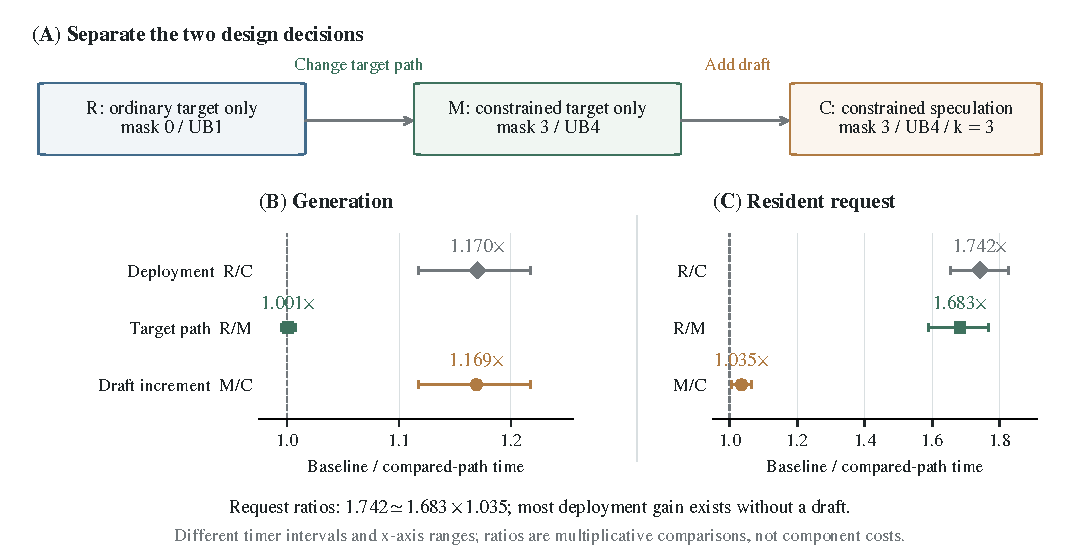
\includegraphics[width=\linewidth]{figures/figure_4_paid_cost.pdf}
\caption{Deployment gain and incremental draft benefit. (A) $R$ is ordinary target-only execution, $M$ the repaired target-only path, and $C$ speculation on that path. (B,C) Geometric means of 24 task ratios formed from four-repetition absolute-time medians; bars show descriptive 95\% task-bootstrap intervals. A ratio above one favors the denominator. Generation and resident-request timers use different intervals and axis ranges. Request ratios satisfy $R/C=(R/M)(M/C)$; this multiplication separates comparisons rather than component costs.}
\label{fig:cost}
\end{figure*}

The identity in Equation~\ref{eq:identity} holds for all 48 task-timer cells and both aggregate timers. Generation $R/M$ is near parity while request $R/M$ is much larger. The target-path change affects prefill microbatch/attention behavior and continuation capacity jointly, and the timer boundaries differ. Their contrast cannot allocate a measured host, attention, KV or synchronization share. A faster qualified ordinary implementation could also narrow the deployment benefit: the registered $R$ is an executed reference, not a proven fastest ordinary decoder.

\subsection{Task variation and session uncertainty}
Figure~\ref{fig:tasks}A,B shows all 24 tasks in the same request-sorted order and scale. Generation improves on 22/24 tasks, but request time improves on only 17/24. Seven tasks regress against matched execution, despite all 24 being faster than ordinary request cost. The average request gain therefore does not justify an unconditional per-task acceleration claim.

The within-round matched-request geometric means in Figure~\ref{fig:tasks}C are 1.029, 0.940, 1.052 and 1.044: round 2 reverses direction. These round summaries differ from the geometric mean formed after taking each task's four-repetition absolute-time medians. The descriptive task-bootstrap interval for that median-based aggregate lies above one, but does not remove the observed round reversal or estimate independent session/day uncertainty.

\begin{figure*}[t]
\centering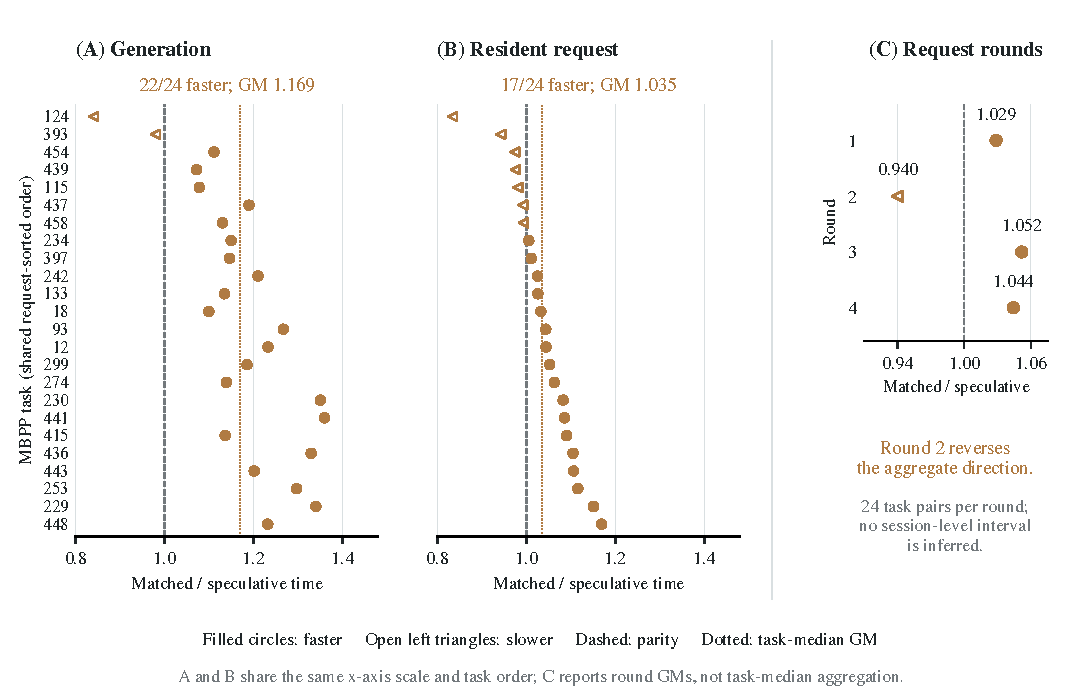
\includegraphics[width=\linewidth]{figures/figure_5_task_variation.pdf}
\caption{Variation behind the matched RTX benefit. (A,B) All 24 tasks share order and scale; ratios use four-repetition absolute-time medians. Generation improves on 22/24 and request time on 17/24. Filled circles denote faster speculation and open left triangles slower speculation, separately for each timer. Dashed lines mark parity; dotted lines mark task-median geometric means. (C) Geometric means within four request rounds, with reversal in round 2. Round summaries are not the task-median estimator or a session-level uncertainty interval.}
\label{fig:tasks}
\end{figure*}

The operating point is qualified and positive in aggregate, with a small, uneven request increment. Separate resident sessions, laptop scheduling and thermal variation can affect that estimate; balanced order and task medians do not eliminate session confounding. The larger generation gain applies to its defined interval rather than replacing the request result. Independent session/day replication would be needed to assess stable deployment acceleration.

A separate serial resident-reset study checks whether the anchor preserves output when reused across requests. Two orders retain the registered reference after target-state reset, with matched generation/request speeds about $1.181\times/1.039\times$. This supports finite reset semantics for the original $k=3$/UB4 recipe, without establishing concurrency, throughput or resident qualification of the widened draft. These rows are not pooled with the expansion.

\subsection{Fixed UB: wider drafting qualifies but becomes slower}
The fixed-UB experiment tests the cost of widening a qualified draft. Unlike the joint $k$/UB geometry sweep, this experiment fixes UB4 and mask 3 while testing $k=3,5,7$ on 24 now-exposed MBPP inputs and four exposed HumanEval probes. Each width qualifies in two repetitions. The highest passing width, $k=7$, is then measured in a separate capture-off arm: four conditions, four repetitions and 448 formal requests. Qualification timings do not select the width by speed.

Relative to $k=3$, $k=7$ gives $0.829\times$ generation and $0.890\times$ request speed. Against matched target-only it gives $0.997\times/0.950\times$, whereas the anchor gives $1.203\times/1.068\times$ in this campaign. Ordinary same-width speculation fails its output gate, so its timing cannot serve as qualified speed evidence. For these inputs and this configuration, the measured anchor is preferable to the wider qualified draft.

Caller reduction does not reduce all recorded work. Drafted tokens rise from 3,528 to 5,392, while accepted draft tokens rise from 2,772 to 3,192. Separate captured qualification sessions record target continuation caller counts falling from 305 to 199 but micrographs increasing from 305 to 397. These counts include their own warmups and forced synchronization; they cannot be divided into formal timing to create a component profile. Micrographs are not CUDA kernel launches, and no unique slowdown component is isolated.

At $k=7$, matched generation/request speed is $0.953\times/0.919\times$ on 24 MBPP inputs and $1.308\times/1.164\times$ on four HumanEval probes. Four exposed probes do not validate an online routing rule. Supplement \S S4.3 retains these partitions and the longer-cap checks under their own timers and panels.

\subsection{B570: repair improves an old path but loses to strong baselines}
The B570 repair's formal four-condition matrix contains 119/120 payloads; old N1's first-round MBPP/400 record is missing after an infrastructure interruption. Its time remains unknown, without imputation or a scientific rerun. Ordinary $R$, matched $M$ and candidate $C$ each have 30 complete responses and 15 two-round task-median pairs. Old-N1 comparisons use 14 complete pairs.

The candidate fails the latency objective against both strong baselines (Table~\ref{tab:b570_cost}). Generation/whole-request speed is $0.283\times/0.201\times$ against ordinary $R$ and $0.286\times/0.206\times$ against matched target-only. Both baselines are faster in every available paired round. The target-only paths are close in cost, with $R/M=0.989\times/0.979\times$; the roughly fivefold candidate request cost is therefore not explained by the target-path consistency constraint alone.

% Generated by scripts/reconstruct.py from frozen exports.
\begin{table}[ht]\centering\small
\caption{B570 paid baseline/candidate task-median ratios. $n$ counts complete two-round task pairs: 15 for $R/C$, $M/C$ and $R/M$, and 14 for old N1/$C$. Gen., Request and Host denote generation, whole request and host-observed time. The missing old-N1 task is not imputed; raw suffix work stays charged.}\label{tab:b570_cost}
\setlength{\tabcolsep}{3pt}
\begin{tabular}{@{}lrrrr@{}}\toprule
Ratio & $n$ & Gen. & Request & Host\\\midrule
$R/C$ & 15 & 0.283 & 0.201 & 0.202\\
$M/C$ & 15 & 0.286 & 0.206 & 0.206\\
Old N1/$C$ & 14 & 3.993 & 2.634 & 2.633\\
$R/M$ & 15 & 0.989 & 0.979 & 0.979\\
\bottomrule\end{tabular}

\end{table}


Against the prior old-N1 frontend, the candidate improves generation/request speed by $3.993\times/2.634\times$ over 14 pairs. That improvement is relative to a slow frontend and does not establish a benefit over ordinary deployment. MBPP/245 also reverses the old-path whole/host request comparison in round 2. Endpoint recovery and aggregate improvement do not guarantee improvement in every round.

The endpoint contract retains all online work. Candidate endpoint IDs total 1,150 while raw IDs total 1,176, with all 26 suffix IDs charged. The records contain 888 drafted and 702 accepted tokens, and target/draft continuation caller-token totals of 1,332/1,362. These quantities describe different parts of the transaction; endpoint equality does not assert raw suffix equality. Removing witness readbacks, an extra context and handoff improves the frontend, but phase reservation, synchronization, drafting and rollback remain. Without a full component profile, the remaining bottleneck cannot be assigned uniquely. The paid decision is to reject this candidate for latency against $R$ and $M$.

\subsection{Global serialization, control, and draft-side limits}
Global serialization can recover output while increasing cost. An earlier RTX arm qualifies 57/57 arrays on 19 exposed tasks but achieves $0.677\times$ target-only speed, with descriptive interval $[0.662,0.692]$ and no task faster. Its synchronized post-prefill-to-slot-release timer includes instrumentation and logging. It is a separate negative operating point, not an earlier point on the expansion's server-generation curve; Supplement \S S6.4 retains the host amendment and preceding V3 stop.

The prospective M4 control campaign has 60 tasks, three conditions, three repeats and 540 requests under a post-prefill contract. Always speculation and Guard each qualify 180/180 direct-ID comparisons. Target-only/Always speed is $1.347\times$, but the paired secondary Guard/Always latency ratio is 1.027, with descriptive interval $[1.013,1.044]$: the measured guard is slower. A hindsight oracle choosing only target-only or Always offers about 0.069\% further geometric-mean latency reduction. This narrow two-action opportunity does not bound intra-request policies; the primary and secondary statistical streams remain distinct (Supplement \S S6.6).

On 358H, CPU/NPU drafting each qualifies 90 direct-ID comparisons but gives $0.734\times/0.352\times$ speed. With measured target work and committed progress fixed, eliminating every other nonnegative cost yields prompt-estimator ceilings of $0.837\times/0.845\times$. Even that idealization needs a uniform target-work reduction of at least 16.28\%/15.52\% to reach parity. Draft-only optimization cannot close this conditional budget; changing the target path or state interface requires new qualification and measurement. These are necessary budgets, not achieved optimizations or an impossibility result for NPUs (Supplement \S S6.7). M4 and 358H inform separate design decisions and do not replicate the RTX repair.
\FloatBarrier

\section{Design Implications and Limits}
\label{sec:implications}
\subsection{Constrain the transaction where evidence warrants it}
The diagnostic distinction guides control placement. A current-path effect motivates constraining verification geometry; a retained-state effect motivates preserving state formation or changing its interface; an interaction requires testing both. The RTX design applies target-phase attention constraints, whereas B570 binds a whole recipe within one context. These are distinct implementations informed by local observations, without a unique kernel diagnosis or an automatic selector.

Own-path shams validate restoration at the tested boundary; crosses reveal local dependence; complete registered-output checks qualify the candidate. B570's unchanged immediate decisions and changed continuation make the last step essential. Cost follows qualification: constraining fewer phases or accepting a wider draft can still fail the performance objective.

\subsection{Use both paid baselines for operating decisions}
The ordinary comparison answers whether the deployment change helps; the matched comparison answers whether adding a draft helps on the repaired path. RTX exposes a substantial draft-free target-path opportunity followed by a modest, uneven request increment. Both values are needed to choose an implementation. A faster qualified ordinary decoder could reduce the former, since the registered $R$ is not a demonstrated optimum.

The measured RTX anchor is preferable to its slower qualified wider draft. For latency, reject the B570 recipe against both strong baselines and avoid adding the measured M4 guard on an assumed control benefit. The 358H conditional budget requires changes to target work or state interfaces beyond draft-only optimization. Each decision follows its own output and timer contract, rather than a pooled hardware ranking.

\subsection{Scope of the evidence}
The repair covers one Qwen3 target/draft family, finite panels and pinned runtime variants. RTX's project-unused panel consists of 24 selected MBPP inputs; unused refers to accessible project history, not training exposure. Changed geometry needs renewed qualification, as the failures demonstrate. No second-family result or preservation guarantee on arbitrary inputs is established.

Discrete agreement is weaker than numerical equivalence. The score/KV witnesses do not separate every reduction, precision, layout or scheduling effect, and shams cannot exhaust hidden backend state. Selected cuts and a four-switch family cannot establish universal minimality. Prior preservation methods were not implemented as same-contract baselines, so superiority over them remains untested.

Task medians and descriptive intervals leave session, thermal and infrastructure variation unresolved. The B570 old-N1 payload and some historical raw comparisons remain missing. Timer and historical energy domains differ; later direct-ID qualification cannot validate earlier text-based timing. The reproducible CPU checks cover included sources and exports, with original-host private-archive audits identified separately in Supplement \S S7.

\section{Conclusion}
Preserving a fixed ordinary greedy output requires a runtime to account for retained state and current execution, then qualify the complete output under an explicit configuration. In the tested RTX implementation, a query-layout change during target prefill and continuation retains other batched work and qualifies a finite full-response panel. Natural crosses motivate that scope, while the complete phase matrix and wider-geometry failures bound it.

Measured cost determines whether the qualified design is useful. The RTX request speed is $1.742\times$ ordinary execution; the draft-free target path already gives $1.683\times$, and speculation adds $1.035\times$ relative to that matched path. The increment is uneven and reverses in one round. A wider qualified draft loses, B570 endpoint repair remains slower than strong baselines, and the auxiliary M4/358H cases constrain the value of added control and draft-only optimization. These findings support local diagnosis, configuration-specific qualification and measurement against both baselines. They do not establish repair beyond the tested Qwen3 family, superiority to external methods under the same contract, or stability across independent sessions.

\section*{Author-review declarations}
\textbf{Authorship and contributions.} Author names, affiliations, corresponding-author details and individual CRediT roles await author confirmation. This draft does not assign authorship or contributions.

\textbf{Funding and competing interests.} Funding sources and competing-interest declarations await confirmation by all authors; absence of a funding source or competing interest is not asserted.

\textbf{Data and software availability.} The author-review source package includes frozen committed evidence exports, source bindings, selected implementation and report records, and CPU-only code for recalculation and figures. Original runtime code and experiment records are retained in the HeteroSpec project. Availability and permitted redistribution of private raw archives, model artifacts and a permanent public data/software location require author confirmation before submission. The supplied exports enable the numerical checks specified in Supplement \S S7; they do not substitute for a full private-archive audit or a rerun of model inference.

\textbf{Declaration of generative AI and AI-assisted technologies in manuscript preparation.} OpenAI ChatGPT/Codex was used to assist with restructuring and drafting text, source and bibliography checks, CPU analysis and plotting code, and the execution-architecture illustration. Quantitative figures are generated from the identified experimental exports, without generative replacement of observations. This author-review version still requires the authors' final scientific, bibliographic and language verification. The final declaration and responsibility statement must be confirmed by the authors before submission.

\bibliographystyle{elsarticle-num}
\bibliography{references}
\end{document}
